\documentclass[../../main.tex]{subfiles}

\begin{document}
\chapter{Linguaggio e semantica}
Un linguaggio di programmazione é un linguaggio formale, ovvero un insieme di simboli e regole che definiscono la struttura e il significato delle istruzioni che compongono un programma.
In questo capitolo definisco il linguaggio che andremo ad utilizzare per descrivere i programmi e la semantica che gli daremo. Il linguaggio é stato pensato per essere comprensibile e allo stesso tempo espressivo, in modo da poter descrivere programmi complessi. La semantica é stata pensata per essere semplice da implementare e allo stesso tempo potente, in modo da poter descrivere programmi complessi.
Un linguaggio viene definito da una grammatica $G = (N, T ,\rightarrow, S)$ dove:
\begin{itemize}
    \item $N$ é l'insieme dei \textbf{non terminali}
    \item $T$ é l'insieme dei \textbf{terminali}
    \item $\rightarrow$ é l'insieme delle \textbf{produzioni}
    \item $S$ é il \textbf{simbolo iniziale}
\end{itemize}

Mentre il linguaggio generato da una grammatica $G$ é definito come:
\begin{equation}
    \mathcal{L}(G) = \{\gamma | \gamma \in T^* \land \Rightarrow^+ w\}
\end{equation}
e $T^*$ é la chiusura di Kleene.\\
La grammatica (che descriveremo nel dettaglio nel capitolo successivo), é riconosciuta dal plugin ANTLR che ci permette di generare un parser per il linguaggio. Il parser generato da ANTLR é un parser LL(*), ovvero un parser che riconosce linguaggi non ambigui e che non richiede backtracking, utilizzando un numero arbitrario di lookahead symbols, questo ci permette di avere un parser efficiente ottimizzando il riconoscimento del linguaggio.

\section{Grammatica}

\subsection{Grammatica del linguaggio}
Di seguito espongo la grammatica del linguaggio \textbf{HLCostLan} che descrive il linguaggio che utilizzeró per descrivere i programmi.\\
Riporto di seguito le produzioni della grammatica che descrivono il linguaggio, mentre per visualizzare il file g4 nella sua totalitá si rimanda alla \href{https://github.com/minosse99/CostCompiler/blob/master/src/HLCostLan.g4}{Repository} del progetto.\\
\label{sec:grammatica}

\begin{lstlisting}[language=ANTLR, caption={Grammatica del linguaggio HLCostLan}, label={lst:grammatica}]
prg : complexType* serviceDecl* functionDecl* init;
    
init: '('formalParams? ')''=''>' '{' stm '}';
    
serviceDecl:'service'ID':''('(type(','type)*)?')''->''type';
    
functionDecl:'fn'ID'('formalParams?')''->'(type)'{'stm'}' ;
    
stm :
    | serviceCall
    |'if''('expOrCall')''{'stm'}''else''{'stm'}'
    |'for''('ID'in''('NUMBER','exp ')'')''{'stm'}'  
    | letIn
    | functionCall
    | 'return' expPlus ;
    
serviceCall:'call'ID'('(exp(','exp)*)?')'(';'stm)?;

functionCall : ID'('( exp (','exp)* )? ')';

letIn: 'let' (ID '=' expPlus)+ 'in' stm;
                                   
    
    \end{lstlisting}
Il non terminale \textbf{prg} e' il terminale iniziale della grammatica, e descrive un programma. Un programma e' composto da una sequenza di dichiarazioni di tipi complessi, dichiarazioni di servizi(che possono avere un overhead in termini di invocazioni che influiscono sul costo), dichiarazioni di funzioni, e infine l'init. L'init e' la funzione che viene invocata all'avvio del programma.
Il non terminale \textbf{init} descrive la funzione init, che deve essere dichiarata una sola volta ed e' composta da una sequenza di parametri formali, e da una istruzioni.\\
La \textbf{serviceDecl} descrive la dichiarazione di un servizio, che deve essere dichiarato una sola volta. Un servizio e' composto da un nome, una sequenza di parametri formali, e un tipo di ritorno.\\
La \textbf{functionDecl} descrive la dichiarazione di una funzione, una funzione e' composta da un nome(univoco), una sequenza di parametri formali, e un tipo di ritorno.
Nel checking semantico controlliamo che non vengano dichiarate due volte funzioni o servizi con lo stesso nome.\\
Inoltre il Type checking controlla che i tipi di ritorno delle funzioni e dei servizi siano corretti.\\


\section{Another Tool for Language Recognition}
ANTLR (Another Tool for Language Recognition) é uno strumento potente e flessibile per l'analisi di linguaggi di programmazione, linguaggi di markup e dati strutturati. é ampiamente utilizzato per generare parser e lexer per vari linguaggi di programmazione e per costruire compilatori, interpreti, traduttori di linguaggi e altre applicazioni che necessitano di analisi di linguaggi.
Ecco alcuni usi comuni di ANTLR:
\begin{enumerate}
    \item Generazione di parser e lexer: ANTLR può generare parser e lexer per molti linguaggi di programmazione, rendendo più semplice l'analisi sintattica e lessicale.
    \item Costruzione di compilatori e interpreti: ANTLR é spesso utilizzato nella costruzione di compilatori e interpreti, poiché fornisce gli strumenti per analizzare il codice sorgente e costruire l'albero di sintassi astratta.
    \item Traduzione di linguaggi: ANTLR può essere utilizzato per tradurre codice da un linguaggio di programmazione a un altro. Questo é utile per la migrazione del codice, la refactoring e altre attivitá di manutenzione del software.
    \item Analisi di dati strutturati: ANTLR può essere utilizzato per analizzare dati strutturati, come file XML o JSON, rendendo più semplice l'estrazione e la manipolazione dei dati.
\end{enumerate}

ANTLR data una grammatica in input, con estensione \textit{.g4}, genera una cartella \textit{gen} contenente i file necessari per generare il parser.\\

\subsection{EBNF: Simboli e notazioni in ANTLR}
I simboli utilizzati da ANTLR, rispettano la notazione EBNF(Extended Backus-Naur Form), che é una notazione formale per descrivere la sintassi di un linguaggio, definita come standard internazionale da ISO-14977.

\begin{itemize}
    \item \textbf{()} - Le parentesi vengono utizzate per raggruppare elementi diversi, e per definire l'ordine di valutazione.
    \item \textbf{?} - i Token seguiti da un punto interrogativo sono opzionali, e possono presentarsi 0 o 1 volta.
    \item \textbf{*} - Chiusura di Kleene, i token seguiti da un asterisco possono presentarsi 0 o piú volte.
    \item \textbf{+} - i token seguiti da un segno piú possono presentarsi 1 o piú volte.
    \item \textbf{|} - il simbolo pipe viene utilizzato per definire una scelta, ovvero un token o un'altro.
    \item \textbf{.} - Il punto definisce che un token puó apparire una singola volta.
    \item \textbf{$\thicksim$ } - Il simbolo not definisce che un simbolo non puó apparire.
    \item \textbf{..} - Il simbolo Range definisce un intervallo di token.
\end{itemize}
L'uso di lettere maiuscole e minuscole é importante, in quanto ANTLR distingue tra token maiuscoli e minuscoli.\\
\autocite{amslaurea2372}

\subsection{Differenza tra Lexer e Parser in ANTLR}
I linguaggi di programmazione sono costituiti da parole chiavi(keywords) e costrutti definiti in modo preciso.
Un file sorgente viene inviato come flusso ad un lexer, carattere per carattere da una qualche interfaccia di input.
Il lexer si occuppa di raggruppare i caratteri in token, ovvero sequenze di caratteri che rappresentano parole chiavi, identificatori, numeri, stringhe, e altri costrutti del linguaggio.
Analogamente al lexer, il parser si occupa di riconoscere la grammatica del linguaggio, dandogli un qualche significato semantico.
La cartella \textit{gen} contiene il codice sorgente del parser e lexel, generati automaticamente; é presente anche un file \textit{.tokens} che contiene i token riconosciuti dal lexer, e un file \textit{.interp} che contiene la tabella di interpretazione del parser.\\
Il lexer si occupa di riconoscere i token, in ANTLR viene generato un lexer DFA, ovvero un lexer che riconosce linguaggi non ambigui e che non richiede backtracking. Questo ci permette di avere un lexer efficiente ottimizzando il riconoscimento del linguaggio.
Il parser, invece, data una sequenza di token, riconosce la grammatica, e genera un albero di parsing(noto anche come albero di derivazione), che rappresenta la derivazione secondo le regole della grammatica libera da contesto. 
Nell'albero di parsing ogni nodo interno corrisponde a una regola della grammatica e ogni foglia corrisponde a un token del linguaggio.
\begin{figure}[H]
    \centering
    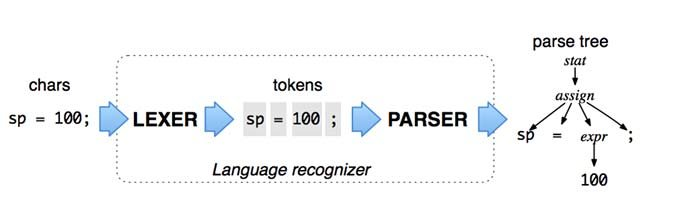
\includegraphics[width=0.9\textwidth]{example_lexer_parser.png}
    \caption{Funzione di parsing e lexing}
\end{figure}
Una volta ottenuto l'albero di parsing possiamo andare a visitarlo, e generare un albero di sintassi astratta, che rappresenta il significato del programma.
L'albero di sintassi astratta(AST) é un albero che rappresenta il significato del programma, e viene utilizzato per eseguire il programma.
A questo punto si estende l'interfaccia \textit{BaseListener} per costruire un albero di sintassi astratta per implementare i metodi necessari per visitare l'albero di parsing e generare l'albero di sintassi astratta.\autocite{antlrllkparser}
\begin{figure}[H]
    \centering
    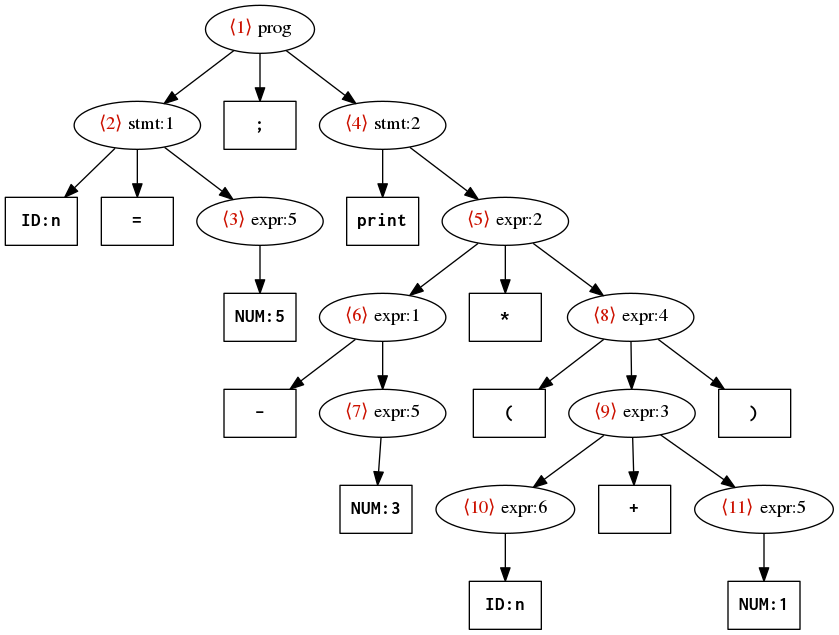
\includegraphics[width=0.9\textwidth]{visit-tree.png}
    \caption{Esempio di albero di AST}
    \label{fig:visit_tree}
\end{figure}

Facciamo un esempio di un frammento di codice realmente generato da ANTLR, per la grammatica \textit{HLCostLan}:
\begin{lstlisting}[language=Java, caption={Esempio di codice HLCostLan: example/Listing6}, label={lst:example_code}]
service BasicService: (int) -> void;
fn svc(i: int) -> void{
    for(m in (0,10)){
        call BasicService(i)
    }

}
(len : int) => {
	svc(len)
}
\end{lstlisting}

Come abbiamo visto nella grammatica \ref{sec:grammatica}, il non terminale \textbf{prg} e' il terminale iniziale della grammatica. In questo caso prg, prende un parametro len di tipo intero, ed avrá un CallNode ad una funzione \textit{svc} che prende un parametro di tipo intero, e ritorna void.\\
La funzione \textit{svc} invece, contiene un for, che itera da 0 a 10, e ad ogni iterazione effettuata una chiamata al servizio \textit{BasicService} con parametro \textit{i}.\\



\section{Semantica del Linguaggio}\label{sec:semantica}
La semantica di un linguaggio di programmazione é l'insieme delle regole che definiscono il significato delle istruzioni, delle espressioni e delle strutture di controllo del flusso nel linguaggio. In altre parole, la semantica definisce ``cosa fa'' un programma scritto in quel linguaggio.

Ad esempio, se definiamo un linguaggio che permette l'assegnamento(non é il nostro caso perché la grammatica HLCostLan non lo permette) dovremmo andare a controllare che la variabile assegnata sia stata dichiarata altrimenti dovrá generare un errore.\\
I controlli semantici del compilatore in oggetto sono di altra natura, quali:
\begin{itemize}
    \item Controllare che non vengano dichiarate due volte funzioni o servizi con lo stesso nome.
    \item Controllare che i parametri utilizzati nelle chiamate di funzioni o servizi siano corretti e quindi giá stati precedentemente dichiarati
    \item Controllare che i tipi di ritorno delle funzioni e dei servizi siano corretti.
\end{itemize}
Inoltre effettuiamo il type checking, che é un sottoinsieme del controllo semantico, che controlla che i tipi delle espressioni siano corretti.\\
\begin{itemize}
    \item I tipi delle chiamate devono essere corretti, ovvero i parametri attuali devono essere dello stesso tipo dei parametri formali.
    \item In un costrutto \textit{let} le espressioni devono essere dello stesso tipo della variabile a cui vengono assegnate.
    \item In un costrutto \textit{if} l'espressione deve essere di tipo booleano, mentre i valori di ritorno degli statemente \textit{then} e \textit{else} devono essere dello stesso tipo.
    \item La funzione deve tornare il tipo dichiarato.
\end{itemize}
\section{Compilatore o Interprete?}
Nel processo di traduzione del codice sorgente in istruzioni eseguibili, due approcci predominanti emergono: il compilatore e l'interprete. Mentre entrambi condividono l'obiettivo di rendere il codice sorgente eseguibile, le loro metodologie differiscono significativamente, portando a implicazioni distinte per le prestazioni, la portabilità e lo sviluppo delle applicazioni software.

Il compilatore adotta un approccio ``one-shot'', traducendo l'intero codice sorgente in un'unica fase e producendo un file eseguibile indipendente dal codice originale. Questo file può essere eseguito più volte senza la necessità di ulteriori traduzioni, garantendo una maggiore efficienza nell'esecuzione del programma. Tuttavia, il processo di compilazione può richiedere più tempo e risorse iniziali, poiché l'intero codice deve essere tradotto prima dell'esecuzione.

D'altra parte, l'interprete adotta un approccio ``line-by-line'', traducendo e eseguendo istruzioni del codice sorgente una alla volta. Questo significa che il codice viene tradotto e eseguito in tempo reale durante l'esecuzione del programma. Sebbene questo approccio possa ridurre il tempo di avvio e la memoria richiesta per l'esecuzione, può comportare una minore efficienza durante l'esecuzione effettiva, poiché le istruzioni devono essere interpretate ad ogni esecuzione.

Nel nostro il plug-in ANTLR diamo in input l'intero file per fare il paring, ma allo stesso tempo generiamo un albero di parsing che viene visitato per generare l'albero di sintassi astratta, che rappresenta il significato del programma, generando però un codice ``intermedio'' per la fase di WebAssembly, mentre per la generazione dell'equazioni di costo, l'output puó essere direttamente un input per un CostAnalyzer come PUBS e CoFloCo.
\autocite{DBLP:books/aw/AhoSU86}


\end{document}
 